\begin{table}
    \centering
    \begin{center}
        \begin{tabular}{lllllll}
        \toprule
        Setting & CoQA & DROP & QuAC & SQuADv2 & RACE-h & RACE-m\\ 
        \midrule
        Fine-tuned SOTA  & \textbf{90.7}\textsuperscript{\textit{a}} & \textbf{89.1}\textsuperscript{\textit{b}} & \textbf{74.4}\textsuperscript{\textit{c}} & \textbf{93.0}\textsuperscript{\textit{d}} & \textbf{90.0}\textsuperscript{\textit{e}} & \textbf{93.1}\textsuperscript{\textit{e}} \\ 
        GPT-3 Zero-Shot  & 81.5 & 23.6 & 41.5 & 59.5 & 45.5 & 58.4 \\
        GPT-3 One-Shot & 84.0 & 34.3 & 43.3 & 65.4 & 45.9 & 57.4 \\
        GPT-3 Few-Shot  & 85.0 & 36.5 & 44.3 & 69.8 & 46.8 & 58.1 \\
        \bottomrule
        \end{tabular}
        \end{center}
    \caption{Results on reading comprehension tasks. All scores are F1 except results for RACE which report accuracy. \textsuperscript{\textit{a}}\cite{ju2019technical} \textsuperscript{\textit{b}}\cite{dropsota} \textsuperscript{\textit{c}}\cite{quacsota} \textsuperscript{\textit{d}}\cite{squadv2sota} \textsuperscript{\textit{e}}\cite{shoeybi2019megatronlm} }
    \label{table:reading_comprehension}
\end{table}
\begin{figure}
\centering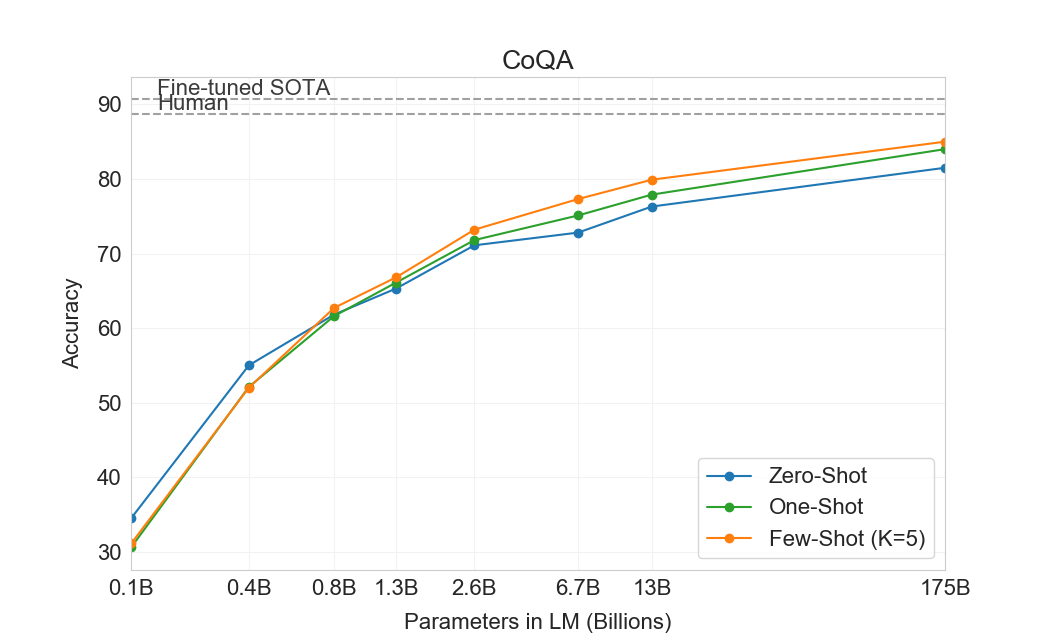
\includegraphics[width=0.8\linewidth]{graphs/scale_plots/coqa.png}
\caption{GPT-3 results on CoQA reading comprehension task.  GPT-3 175B achieves 85 F1 in the few-shot setting, only a few points behind measured human performance and state-of-the-art fine-tuned models.  Zero-shot and one-shot performance is a few points behind, with the gains to few-shot being largest for bigger models.}
\label{graph:coqa}
\end{figure}
Next we evaluate GPT-3 on the task of reading comprehension. We use a suite of 5 datasets including abstractive, multiple choice, and span based answer formats in both dialog and single question settings. We observe a wide spread in GPT-3's performance across these datasets suggestive of varying capability with different answer formats. In general we observe GPT-3 is on par with initial baselines and early results trained using contextual representations on each respective dataset.

GPT-3 performs best (within 3 points of the human baseline) on CoQA \cite{reddy2019coqa} a free-form conversational dataset and performs worst (13 F1 below an ELMo baseline) on QuAC \cite{choi2018quac} a dataset which requires modeling structured dialog acts and answer span selections of teacher-student interactions. On DROP \cite{dua2019drop}, a dataset testing discrete reasoning and numeracy in the context of reading comprehension, GPT-3 in a few-shot setting outperforms the fine-tuned BERT baseline from the original paper but is still well below both human performance and state-of-the-art approaches which augment neural networks with symbolic systems \cite{ran2019numnet}. On SQuAD 2.0 \cite{rajpurkar2018know}, GPT-3 demonstrates its few-shot learning capabilities, improving by almost 10 F1 (to 69.8) compared to a zero-shot setting. This allows it to slightly outperform the best fine-tuned result in the original paper. On RACE \cite{lai2017race}, a multiple choice dataset of middle school and high school english examinations, GPT-3 performs relatively weakly and is only competitive with the earliest work utilizing contextual representations and is still 45\% behind SOTA.
